%---------- Inleiding ---------------------------------------------------------

% TODO: Is dit voorstel gebaseerd op een paper van Research Methods die je
% vorig jaar hebt ingediend? Heb je daarbij eventueel samengewerkt met een
% andere student?
% Zo ja, haal dan de tekst hieronder uit commentaar en pas aan.

%\paragraph{Opmerking}

% Dit voorstel is gebaseerd op het onderzoeksvoorstel dat werd geschreven in het
% kader van het vak Research Methods dat ik (vorig/dit) academiejaar heb
% uitgewerkt (met medesturent VOORNAAM NAAM als mede-auteur).
% 

\section{Inleiding}%
\label{sec:inleiding}

In de recente ontwikkeling van IoT apparaten, zoals bewakingscamera's, sensoren, slimme tv's, printers enzoverder, neemt de behoefte om deze te beveiligen immer toe \autocite{Matter2024}. Bedrijven maken steeds vaker gebruik van zulke apparaten met een internetcapaciteiten om hun productiviteit te verhogen. 

Helaas zorgt dit voor uitdagingen op het gebied van cyberbeveiliging. Veel van deze gadgets kunnen door cyberaanvallers worden gezien als toegangspunten tot onze netwerken \autocite{Hodes2024}. 

Dit onderzoek richt zich op het evalueren en optimalisatie van open-source Intrusion Detection Systems (IDS), zoals Suricata en Zeek, binnen een gesimuleerde IoT-omgeving die representatief is voor een klein bedrijf. Dit onderzoek is van groot belang om kleine bedrijven te helpen hun netwerk beter te beheren door middel van praktische oplossingen die resource zuinig zijn, schaalbaar en doeltreffend zijn, zonder hoge kosten voor commerciële producten of licenties. Dit maakt dit onderzoek niet alleen relevant, maar ook toepasbaar voor een breed scala aan organisaties

Om de onderzoeksvraag te beantwoorden: \emph{“Hoe kan men Suricata en Zeek als intrusion detection systems (IDS) optimaliseren voor een gesimuleerde IoT omgeving in een klein bedrijf met nadruk op resourcegebruik (CPU/geheugen), vlotte schaalbaarheid en detectienauwkeurigheid?”} moeten er een aantal deelvragen worden geformuleerd:


\begin{enumerate}
    \item Wat zijn de meest voorkomende cyberdreigingen bij IoT-apparaten voor kleine bedrijven?
    \item Welke soorten IoT-apparaten en netwerkdreigingen zijn typisch voor kleine bedrijven?
    \item Wat is het gemiddelde resourcegebruik van Suricata en Zeek bij lightweight hardware?
    \item Welke configuraties van Suricata en Zeek minimaliseren resourcegebruik in IoT-netwerken?
    \item Hoe eenvoudig zijn Suricata en Zeek te implementeren en beheren binnen een IoT-netwerk in een klein bedrijf?
    \item Hoe presteren Suricata en Zeek bij toename van het aantal IoT-apparaten?
    \item Wat is de detectienauwkeurigheid van Suricata versus Zeek bij het identificeren van IoT-dreigingen?
\end{enumerate}

Om deze vragen te beantwoorden, zullen beide IDS-en getest worden in een gesimuleerde omgeving de kenmerkend is voor een klein bedrijf met IoT-toestellen, dus een Proof-of-Concept (PoC). Hierbij worden de resultaten van beide IDS geëvalueerd op basis van hun detectievermogen, resourceverbruik en implementatiegemak.

De resultaten van dit onderzoek zetten netwerkbeheerders aan om een doordachte keuze tussen Suricata en Zeek als geschikte IDS-oplossing wanneer er kwaadaardige of ongeautoriseerde activiteiten plaatsvinden voor hun specifieke use case.


%---------- Stand van zaken ---------------------------------------------------

\section{State of the art}%
\label{sec:literatuurstudie}

\subsection{De groei van IoT in bedrijven}

Het aantal aangesloten IoT-apparaten groeit met 14\% in 2025, tot een totaal van 21,1 miljard apparaten wereldwijd, volgens IoT Analytics-analist Satyajit \textcite{Sinha2025}. Eind 2024 waren er 18,6 miljard verbonden IoT-apparaten, wat alleen maar aantoont dat deze stijgende trend de komende jaren zal doorzetten. \\

\begin{figure}[h]
	\centering
	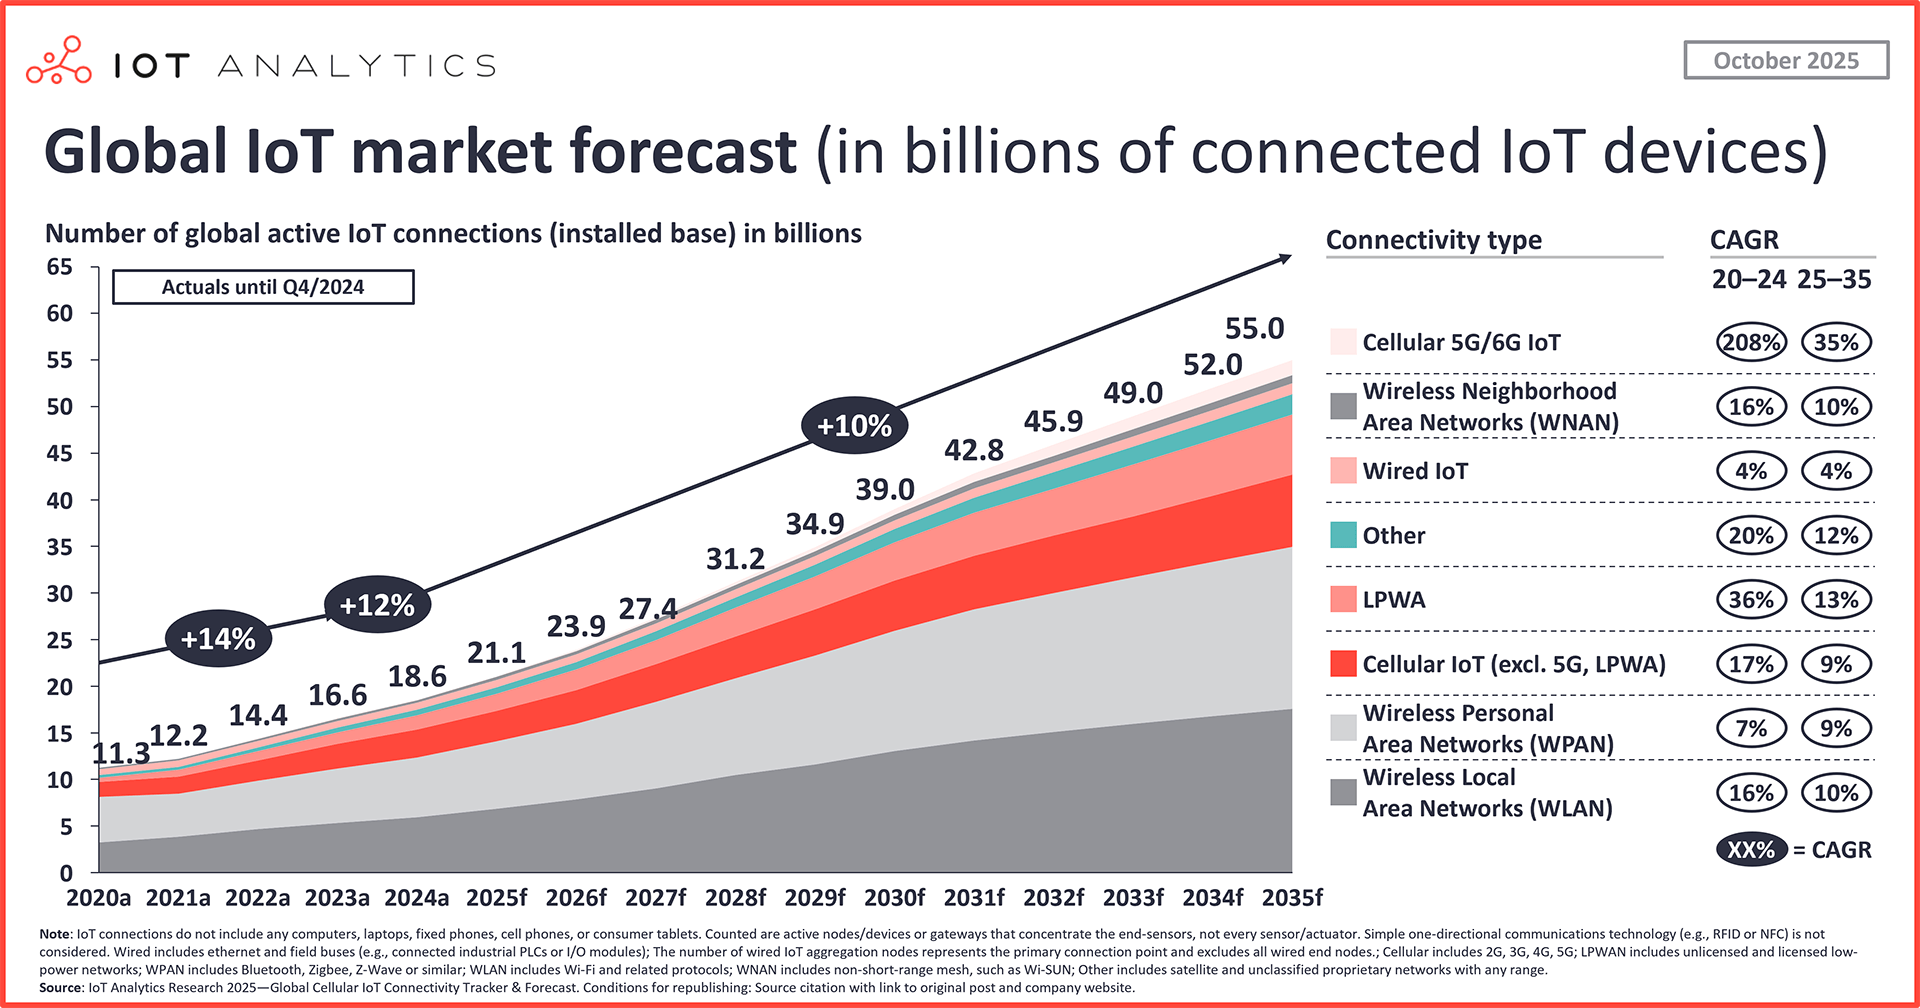
\includegraphics[width=0.5\textwidth]{../graphics/Number-of-connected-IoT-devices-October-2025-vf-vw.png}
	\caption{Voorspelling van de groei van het aantal IoT-toestellen (2020-2035)}
\end{figure}

Het Internet of Things, ook bekend als IoT, verwijst naar een systeem van onderling verbonden apparaten en sensoren die gegevens kunnen verzamelen en delen. Deze gegevens kunnen worden gebruikt om verschillende taken en processen te controleren en te automatiseren \autocite{KinzaYasar2024}. Voorbeelden hiervan zijn slimme thermostaten die de temperatuur controleren of beveiligingscamera’s die een melding sturen wanneer er beweging wordt gedetecteerd. \\

Met de toenemende adoptie van IoT, worden er nieuwe mogelijkheden ontdekt om de automatisering en datagestuurde besluitvorming te verbeteren, waardoor er behoefte ontstaat aan veilige oplossingen om deze netwerken te beheren.


\subsection{De nood aan beveiliging}

De groei van het Internet of Things biedt niet alleen voordelen, maar brengt ook nog veel beveiligingsuitdagingen met zich mee. Zoals Rens \textcite{Braak2024} aangeeft, biedt zelfs het eenvoudigste IoT-apparaat meerdere entry points tot onze infrastructuur.

De meest voorkomende IoT-kwetsbaarheden zijn:

\begin{enumerate}
    \item Zwakke/gecodeerde wachtwoorden
    \item Onveilige netwerken
    \item Onveilige updatemechanismen
    \item Onveilige of verouderde componenten
\end{enumerate}

Deze lijst benadrukt alleen maar de noodzaak van robuuste beveiligingsmaatregelen. Een belangrijk onderdeel hiervan is het gebruik van Intrusion Detection Systems (IDS), die kunnen helpen om deze problemen te detecteren, en indien aanwezig kan een Intrusion Prevention Systems (IPS) de gedetecteerde aanvallen actief blokkeren.

\subsection{Intrusion Detection Systems (IDS)}

Intrusion Detection Systems (IDS) is een netwerk controlesysteem dat oorspronkelijk werd ontwikkeld voor het detecteren van kwetsbaarheden die worden uitgebuit tegen een doelapplicatie of -computer. Dit systeem luistert alleen, observeert het verkeer in realtime en waarschuwt de beheerder als er een kwaadaardige activiteit of ongeautoriseerde toegang heeft plaatsgevonden \autocite{IBM2023}. 

De meest voorkomende soorten IDS kunnen als volgt worden beschreven:
\begin{itemize}
    \item Network-based intrusion detection system (NIDS)
    \item Host-based intrusion detection system (HIDS)
\end{itemize}

Het verschil tussen deze twee is dat NIDS wordt ingezet op de hele infrastructuur, terwijl HIDS wordt ingezet op de doelcomputer die we willen monitoren \autocite{ Data2023}. 


% Voor literatuurverwijzingen zijn er twee belangrijke commando's:
% \autocite{KEY} => (Auteur, jaartal) Gebruik dit als de naam van de auteur
%   geen onderdeel is van de zin.
% \textcite{KEY} => Auteur (jaartal)  Gebruik dit als de auteursnaam wel een
%   functie heeft in de zin (bv. ``Uit onderzoek door Doll & Hill (1954) bleek
%   ...'')



%---------- Methodologie ------------------------------------------------------
\section{Methodologie}%
\label{sec:methodologie}

\begin{itemize}
    \item \textbf{Literatuurstudie en Contextanalyse:} De eerste stap van dit onderzoek begint met het grondig bestuderen van bestaande literatuur om de context van een IoT-omgeving voor een klein bedrijf beter te begrijpen en om het nut van het vooropgestelde onderzoek in deze bacPr0 te verantwoorden. Woorden er use casestudies en real-world implementaties van Suricata en Zeek in IoT-omgevingen gereviewd. Op basis van deze analyse identificeert men de verschillende componenten in zo’n omgeving te identificeren en op te lijsten. Dit omvat het herkennen van veelvoorkomende netwerkdreigingen en een evaluatie van bestaande IDS-oplossingen, zoals Suricata en Zeek.
    
    \item \textbf{Testopstelling Proof of Concept (PoC) Ontwerp:} Op basis van de verzamelde inzichten wordt een gesimuleerde IoT-omgeving opgezet die representatief is voor een klein bedrijf. Hier zullen wij verschillende IoT-apparaten (zoals camera’s, printers, enzoverder) gebruiken om een breder scala aan dreigingen en gebruikssituaties na te bootsen. De IDS zullen worden geïnstalleerd op resourcebeperkte systemen zoals een Intel NUC of een Raspberry Pi om hun doeltreffendheid te meten in een typische low-kost hardware setting.
    
    \item \textbf{Optimalisatie en Testscenario’s:} 
    \begin{itemize}
        \item \textbf{Optimalisatie:} Suricata en Zeek worden aangepast aan de specifieke vereisten van IoT-netwerken om efficiëntie te verbeteren.
        \item \textbf{Scenario’s:} Testen worden uitgevoerd met realistische dreigingen, zoals DoS-aanvallen, port scans, en versleuteld verkeer, om hun prestaties te evalueren.
    \end{itemize}
    
    \item \textbf{Gegevensverzameling en Analyse:} Belangrijke statistieken, zoals CPU- en geheugengebruik, detectienauwkeurigheid, schaalbaarheid en responstijden, worden verzameld. Deze data worden geanalyseerd en gevisualiseerd in tabellen en grafieken.
    
    
    \item \textbf{Meetcriteria:} De prestaties van Suricata en Zeek worden geëvalueerd aan de hand van de volgende criteria:
    \begin{enumerate}
        \item \textbf{Detectienauwkeurigheid:} Het percentage correcte detecties van bedreigingen (True Positives) en het aantal valse meldingen (False Positives).
        \item \textbf{Resourcegebruik:} Meting van CPU-, geheugen- en netwerkgebruik tijdens de uitvoering van de testscenarios.
        \item \textbf{Schaalbaarheid:} De prestaties van de IDS bij een toenemend aantal IoT-apparaten en netwerkverkeer.
        \item \textbf{Reactiesnelheid:} De tijd die de IDS nodig heeft om aanvallen te detecteren en rapporteren.
    \end{enumerate}
    

    
    \item \textbf{Vergelijking en Aanbevelingen:} De resultaten worden vergeleken om inzicht te geven in welke IDS het meest geschikt is voor kleine IoT-netwerken. De analyse biedt praktische aanbevelingen voor het optimaliseren van IDS-configuraties in resource-beperkte omgevingen.
\end{itemize}


%---------- Verwachte resultaten ----------------------------------------------
\section{Verwacht resultaat, conclusie}%
\label{sec:verwachte_resultaten}

Mijn hypothese is dat Suricata beter zal presteren dan Zeek op het gebied van resourcegebruik, zoals CPU-gebruik en geheugenefficiëntie. Suricata zal ook eenvoudiger te implementeren en configureren zijn binnen IoT-netwerken, waardoor het toegankelijker wordt voor kleine bedrijven. Daarom is een proof of concept nodig om mijn hypothese te evalueren en te ondersteunen. Dit onderzoek zal kleine bedrijven ook inzicht geven in het optimaliseren van IDS-implementatie voor IoT-netwerken. 




